\subsection{Casos de test}

Para comenzar el análisis sobre el tiempo de ejecución de cada uno de los métodos, decidimos inicialmente estudiar cómo se comportan frente a los test de la cátedra. %A partir de los resultados logramos obtener mayor claridad sobre cómo se desenvuelven. 
%Esto nos permitirá desarrollar una intuición para realizar un estudio más profundo.

\vspace{2em}
\noindent\textsc{Metodología}. Se realizó el cálculo de \textit{PageRank} sobre la implementación que utiliza la \textit{eliminación gaussiana}, con $\varepsilon = 10^{-6}$, y se calculó $||x - pagerank(g, p)||_1$ donde $x$ refiere a la solución verdadera provista por cada uno de los tests. Cabe destacar que este es un proceso determinístico. 

A partir de este resultado realizamos una búsqueda de la tolerancia ideal, para el \textit{método de Jacobi} y el \textit{método de Gauss-Seidel}, que nos permitiera calcular \textit{PageRank} con un error similar al obtenido anteriormente. Para esto, se realizó ---para ambos métodos--- un binary-search donde en cada paso alteramos la tolerancia $t$ y calculamos el resultado de \textit{PageRank}. Editamos los límites de la tolerancia acorde a si el error calculado fue mayor o menor al error que se cometió con la \textit{eliminación gaussiana}. Repetimos el proceso hasta que la diferencia entre ambas soluciones fue menor a $10^{-2} \times \varepsilon$ en norma $L_1$. %Al finalizar este procedimiento obtuvimos tolerancias tales que, al calcular el error de comparar las respuestas que conceden \textit{Jacobi} y \textit{Gauss-Seidel} con la original, sea similar, en orden de magnitud, al error entre la respuesta que retorna PageRank y la original. 

%De este modo se espera realizar una comparación de tiempo de ejecución justa, donde todos los métodos obtengan una respuesta comparable en términos del error cometido.

%\vspace{1em}
Dados estos parámeteros, se procedió a calcular \textit{PageRank} para cada test, sobre cada implementación y medir el tiempo de ejecución de la etapa de resolución del sistema lineal asociado. Repetimos este paso diez veces para atenuar las fluctuaciones de tiempo de ejecución\footnote{Para evitar disparidades sobre los resultados de este experimento, y el subsiguiente, aclaramos que estos se ejecutaron en una misma computadora.}. 

\vspace{2em}
\noindent \textsc{Resultados}. Procedemos a detallar los resultados en la Figura (\ref{tiempo_ej}.). 

\begin{figure}[!htbp]
    %\ContinuedFloat
    \centering
    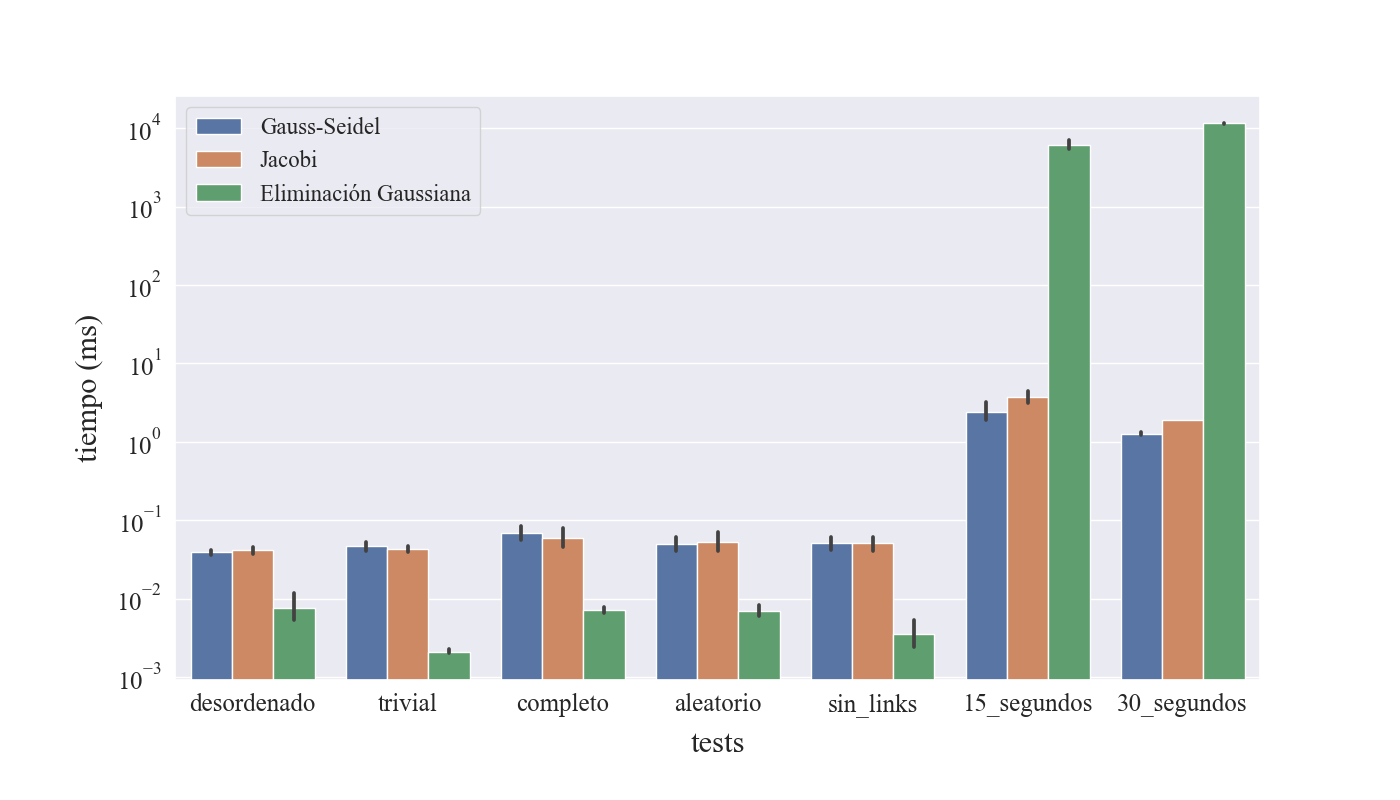
\includegraphics[width=.9\textwidth, trim=0 0 0 30]{files/src/.media/tiempo-ejecucion.png}
    \caption{Tiempo de ejecución ---en milisegundos--- de las distintas implementaciones de \textit{PageRank} para cada uno de los tests de la cátedra (escala logarítmica).} \label{tiempo_ej}
\end{figure}


\vspace{1em}
Como se puede apreciar en el gráfico, el \textit{método de Gauss-Seidel} y el \textit{método de Jacobi} son considerablemente más rápidos cuando el tamaño de la matriz es grande. Para el test \textit{30\_segundos}, estos métodos tardaron alrededor de dos milisegundos, mientras que la \textit{eliminación gaussiana} tardó mas de ocho segundos. Sin embargo, cuando el tamaño de la matriz es chico, notamos que la \textit{eliminación gaussiana} es más rápida. 

\vspace{1em}
Por su parte, los métodos iterativos tienen una velocidad muy similar. El \textit{método de Gauss-Seidel} fue apenas más rápido que el \textit{método de Jacobi} en todos los casos evaluados.


% DENSIDADES
\vspace{2em}
\subsection{En función de la densidad del grafo de entrada}

Más allá de los tests de la cátedra se debe evaluar el comportamiento de los métodos propuestos en función de sistemas alternativos.
Podriamos esperar que el rendimiento de nuesta solución varie con el comportamiento inherente a cada grafo. 
Para poner esto en práctica vamos a generar un conjunto de distintas entradas y analizar su comportamiento en virtud a su densidad.
Es decir, dado ciertas familias de grafos (ver figura \ref{familias}), producimos instancias aleatorias donde podemos variar la proporción entre su cantidad de aristas (links) y nodos.
Buscamos obtener una mejor idea de como se comportan nuestros algoritmos.

\begin{figure}[h]
    \centering
    \subfloat[Aleatorio]{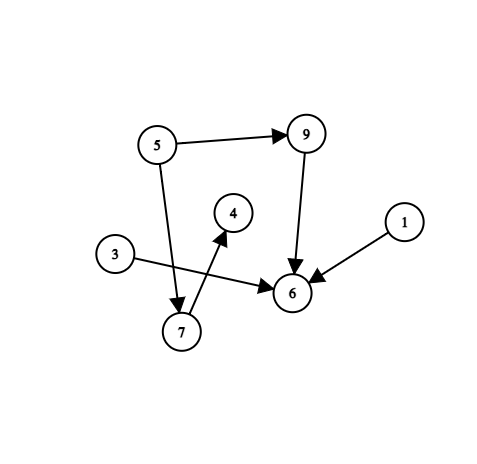
\includegraphics[width=0.3\textwidth]{files/src/.media/familia_aleatorio.png}}
    \subfloat[Red sumidero]{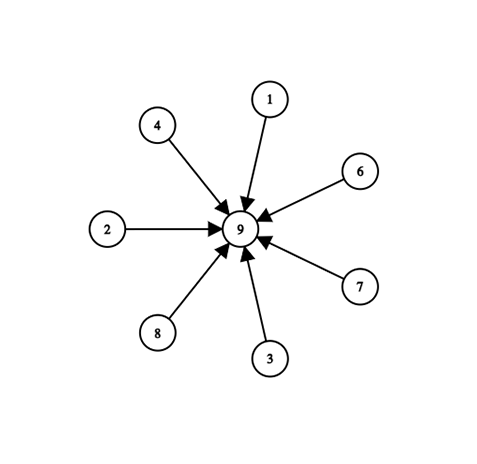
\includegraphics[width=0.3\textwidth]{files/src/.media/familia_red_sumidero.png}}
    \subfloat[Todo con todo]{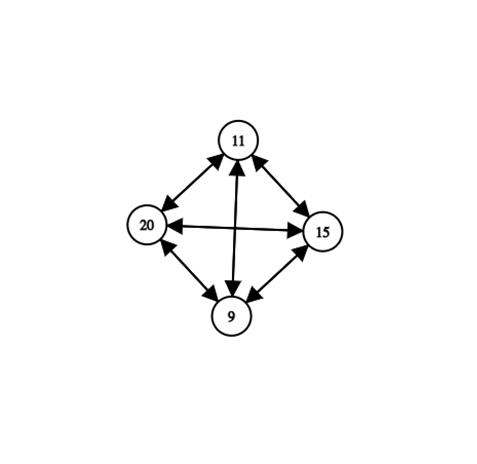
\includegraphics[width=0.3\textwidth]{files/src/.media/familia_todo_con_todo.png}}
    \newline
    \subfloat[Uno a todos]{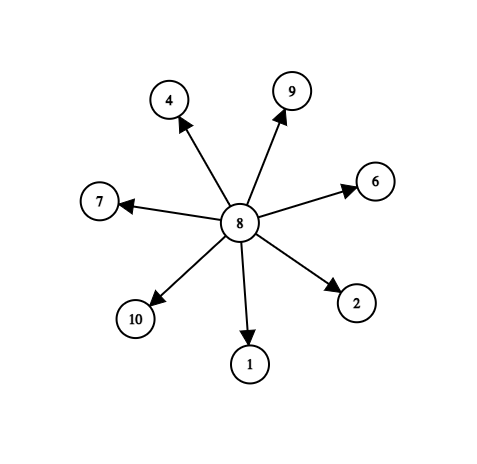
\includegraphics[width=0.3\textwidth]{files/src/.media/familia_uno_con_todo.png}}
    \subfloat[Viborita]{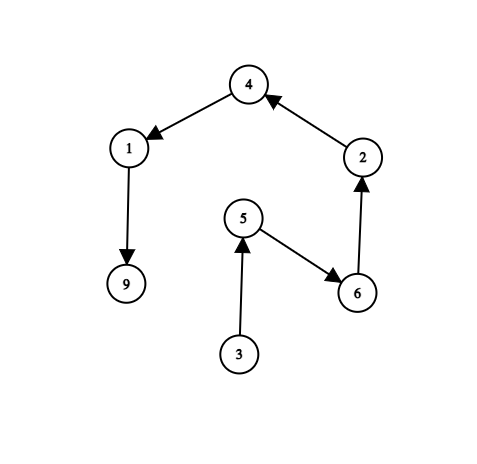
\includegraphics[width=0.3\textwidth]{files/src/.media/familia_viborita.png}}
    \caption{Ejemplos de las familias de grafos generadas para el análisis de densidad.}
    \label{familias}
\end{figure}

\noindent\textsc{Metodología}.
En seguimiento de la sección anterior, atentamos a reconstruir la misma metodología.
Para cada familia de grafos generamos 7 instancias aleatorias, con densidad creciente $d \in \{0.01, 0.05, 0.1, 0.3, 0.5, 0.9, 1\}$.
Estas muestras son aleatorias en vista de que los $N$ nodos que participan de dicha construcción se seleccionan al azar.
Dado un $N$ grande podemos prever una descripción ejemplar de cada categoría. %exceptuando casos extraordinarios donde el arreglo de valores en la matriz de entrada sea especial.
Para \textit{PageRank} usamos nuevamente la tolerancia $\varepsilon = 10^{-6}$.
En búsqueda de una tolerancia justa para los otros dos métodos, desarrollamos el binary-search haciendo uso del error relativo $||Ax - x||_1$,
para el resultado $x$ de cada recursión. 

Con $N = 1000$, se itera por cada $d$ y por cada familia de grafos. En cada caso, experimentamos con cada uno de los tres métodos, generando 10 instancias de grafos distintos.
De estas 1050 muestas construimos los resultados. 

\vspace{2em}
\noindent\textsc{Resultados}.

A simple vista, confirmamos la conclusión de la sección previa: los métodos iterativos son considerablemente más rápidos que la eliminación gaussiana.

El caso de las redes aleatorias (figura \ref{densidad_aleatorio}) pone en manifiesto el comportamiento generalmente esperado: 
el tiempo de ejecución crece en proporción a la densidad del grafo.
Los tres métodos mantienen prolijamente su eficiencia relativa.
Este comportamiento se refleja también en el resto de las figuras, si bien pierden esta misma nitidez.
Es decir, la precedencia de cada método se mantiene en general, pero no siempre es tan clara como en el caso de los grafos aleatorios.
La red sumidero (figura \ref{densidad_red_sumidero}) y el grafo de "uno a todos" (figura \ref{densidad_uno_a_todos}), en particular,
demuestran tiempos de ejecución muy similares para \emph{Jacobi} y \emph{Gauss-Seidel}.
En ambos, el crecimiento de la densidad afecta en gran parte a la \emph{eliminación gaussiana}, pero solo levemente a los métodos iterativos.
También, cabe destacar la variación inesperada para matrices particularmente ralas, como podemos notar en la red sumidero y viborita (\ref{densidad_viborita}).
Por el otro lado, para un grafo completamente conectado (figura \ref{densidad_todo_con_todo}), la distinción es clara; Gauss-Seidel es el más rápido, siempre.

Lo que se puede concluir de estos resultados es la pertinencia de la estructura del grafo que se está analizando.
El comportamiento temporal de los métodos propuestos es muy dependiente de esta, de tal manera que
producir una estimación de su eficiencia podría requerir un estudio puntual al caso.
No obstante destacamos, como regla de oro, el predominio del método de Gauss-Seidel sobre los otros dos.
Donde, incluso si no el más rápido, exhibe poca desventaja sobre el resto.

\begin{figure}[!htbp]
    \centering
    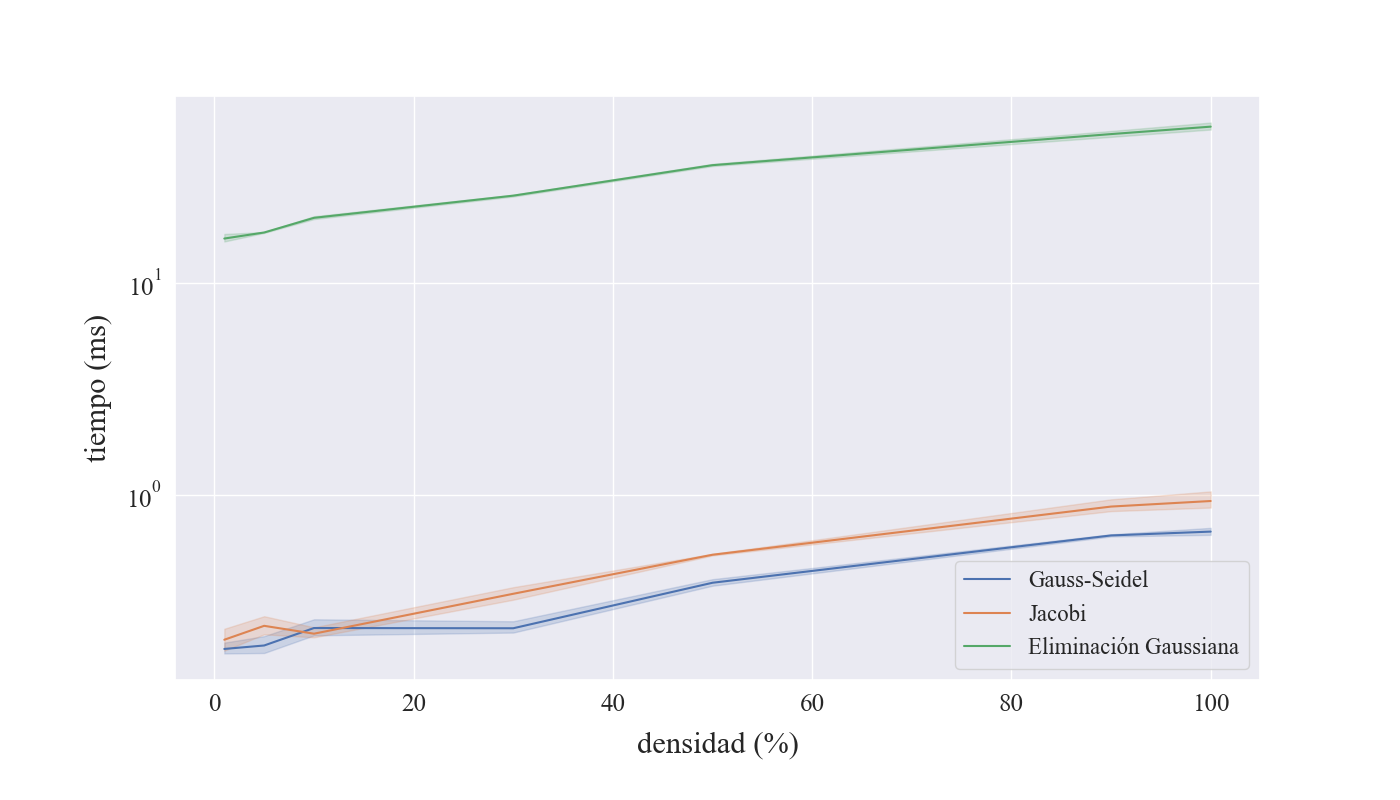
\includegraphics[width=1\textwidth, trim=0 0 0 30]{files/src/.media/densidad_aleatorio.png}
    \textbf{Aleatorio}\par
    \caption{Tiempo de ejecución para el conjunto aleatorio de grafos, con $n = 1000$ y $p = 0.5$, en función de la densidad de conexiones, para cada implementación de \textit{PageRank}.}
    \label{densidad_aleatorio}
\end{figure}

\begin{figure}[!htbp]
    \centering
    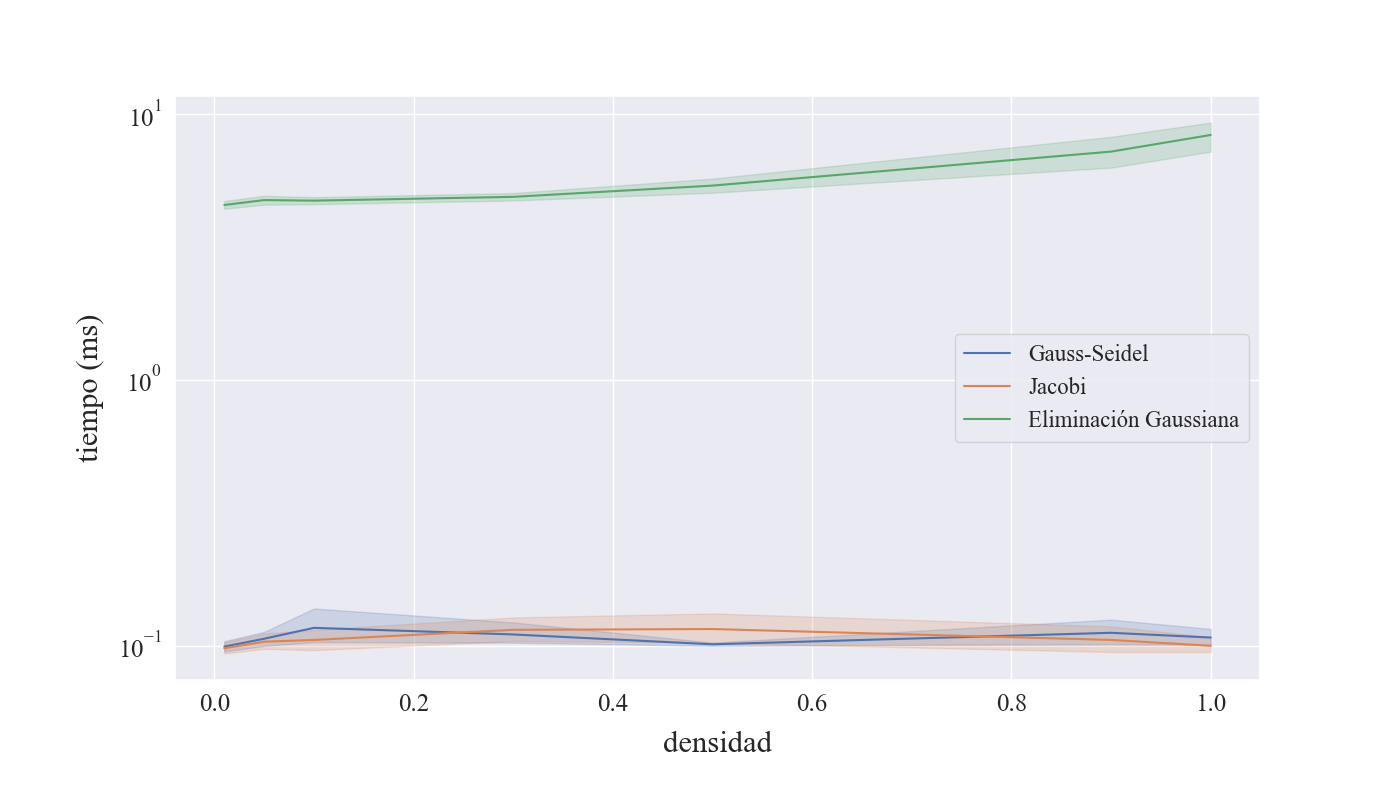
\includegraphics[width=1\textwidth, trim=0 0 0 30]{files/src/.media/densidad_red_sumidero.png}
    \textbf{Red sumidero}\par
    \caption{Tiempo de ejecución para el conjunto de redes sumidero, con $n = 1000$ y $p = 0.5$, en función de la densidad de conexiones, para cada implementación de \textit{PageRank}.}
    \label{densidad_red_sumidero}
\end{figure}

\begin{figure}[!htbp]
    \centering
    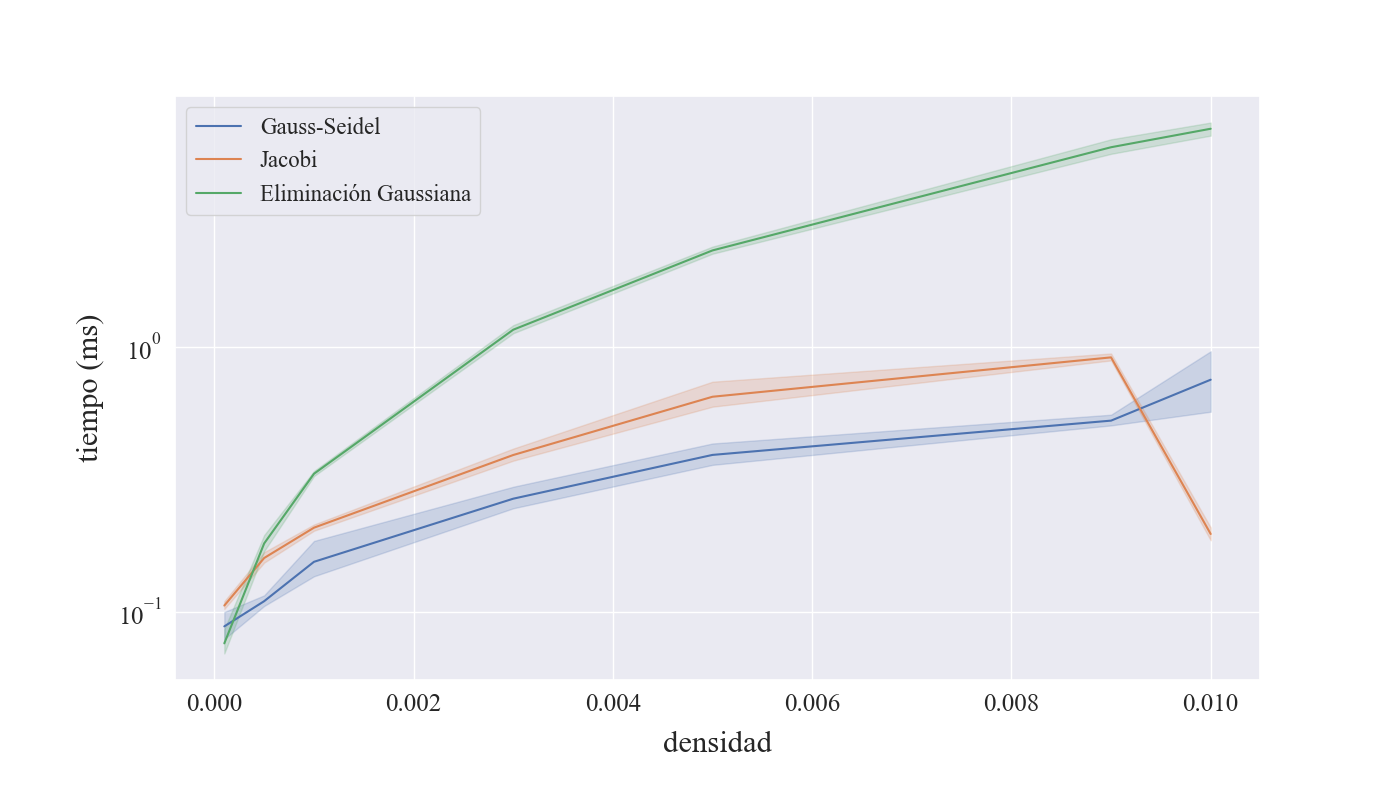
\includegraphics[width=1\textwidth, trim=0 0 0 30]{files/src/.media/densidad_todo_con_todo.png}
    \textbf{Todo con todo}\par
    \caption{Tiempo de ejecución para el conjunto de grafos que conecta cada nodo con todos los demas, con $n = 1000$ y $p = 0.5$, en función de la densidad de conexiones, para cada implementación de \textit{PageRank}.}
    \label{densidad_todo_con_todo}
\end{figure}

\begin{figure}[!htbp]
    \centering
    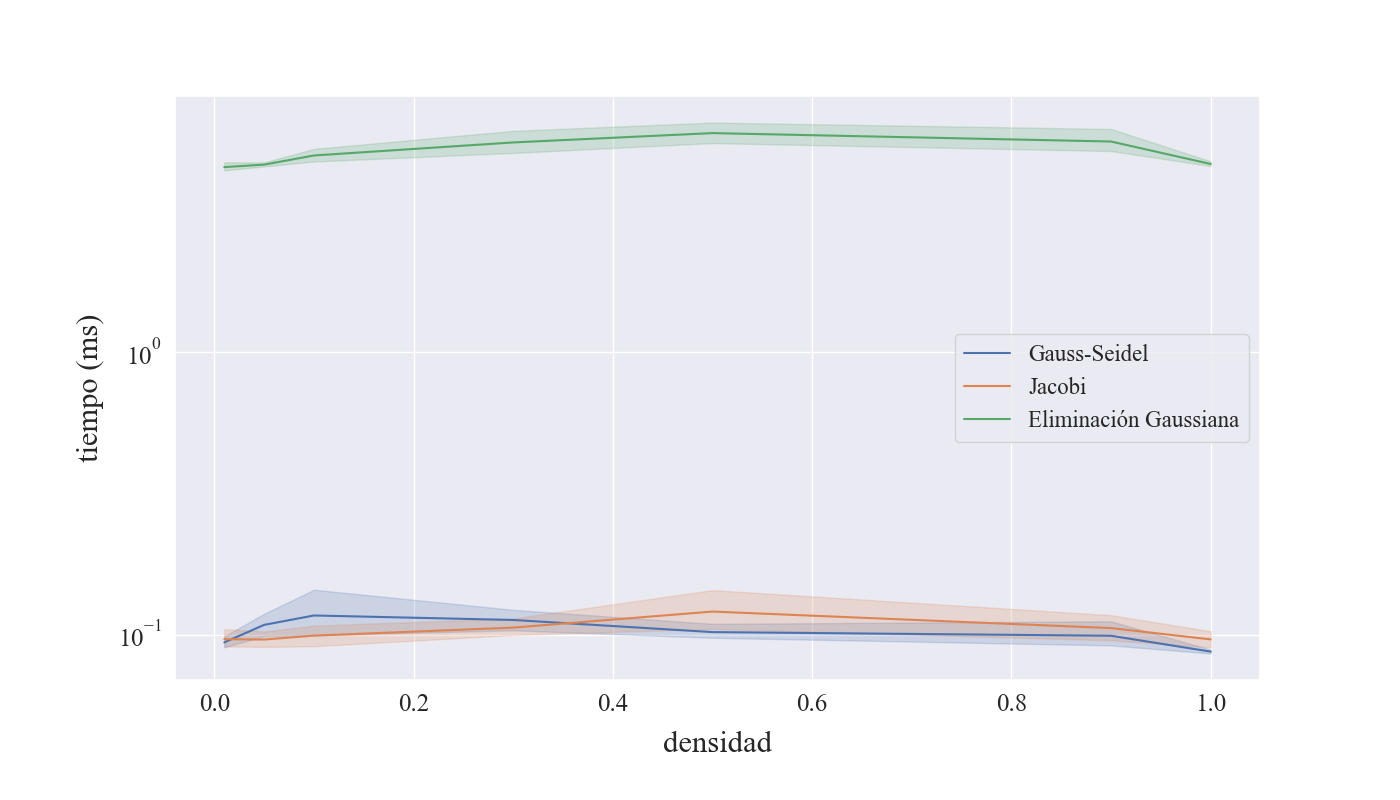
\includegraphics[width=1\textwidth, trim=0 0 0 30]{files/src/.media/densidad_uno_a_todos.png}
    \textbf{Uno a todos}\par
    \caption{Tiempo de ejecución para el conjunto de grafos que conecta un nodo con todos los demas, con $n = 1000$ y $p = 0.5$, en función de la densidad de conexiones, para cada implementación de \textit{PageRank}.}
    \label{densidad_uno_a_todos}
\end{figure}

\begin{figure}[!htbp]
    \centering
    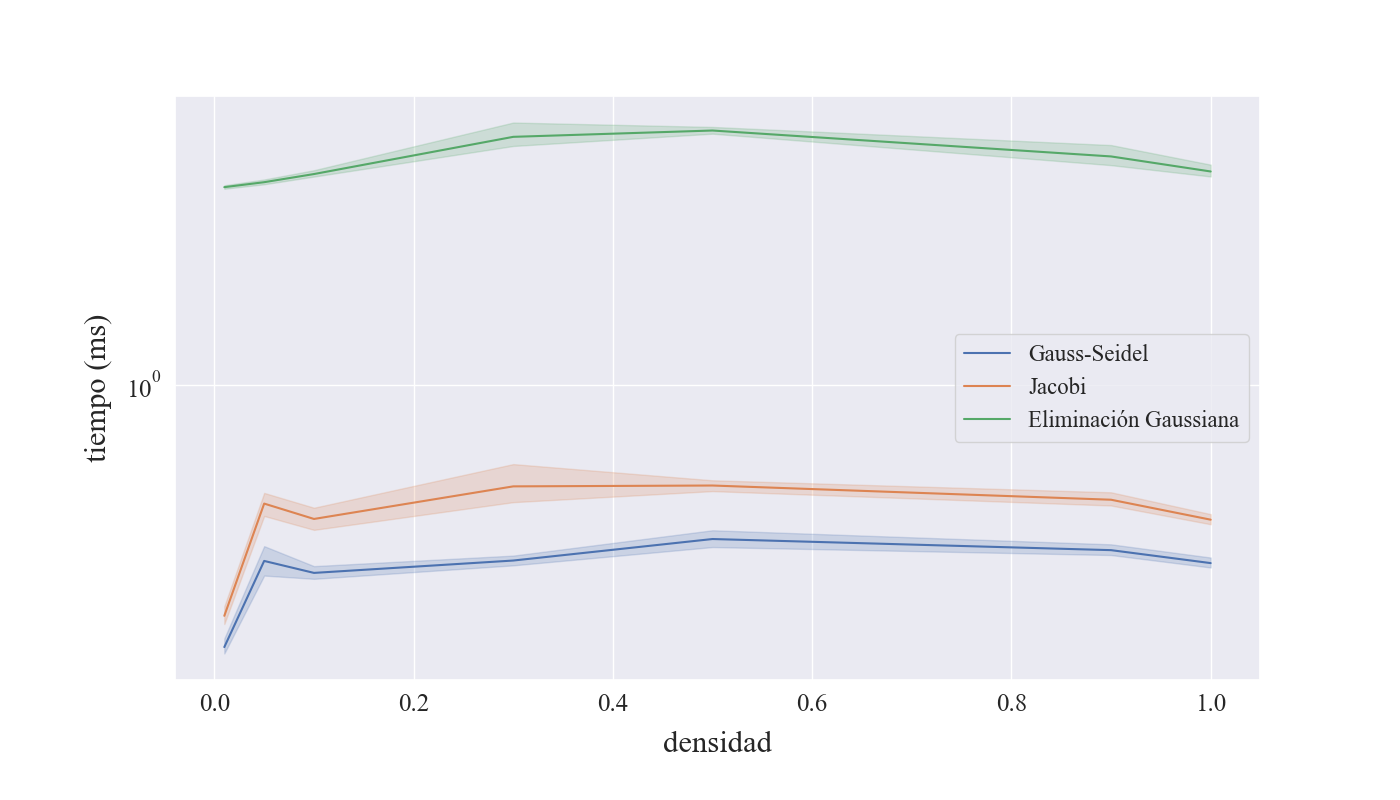
\includegraphics[width=1\textwidth, trim=0 0 0 30]{files/src/.media/densidad_viborita.png}
    \textbf{Viborita}\par
    \caption{Tiempo de ejecución para el conjunto de redes "viborita", con $n = 1000$ y $p = 0.5$, en función de la densidad de conexiones, para cada implementación de \textit{PageRank}.}
    \label{densidad_viborita}
\end{figure}
